\begin{figure}[htbp]
\section*{ NBAS}
\centering
\begin{subfigure}[b]{0.5\textwidth}
\centering
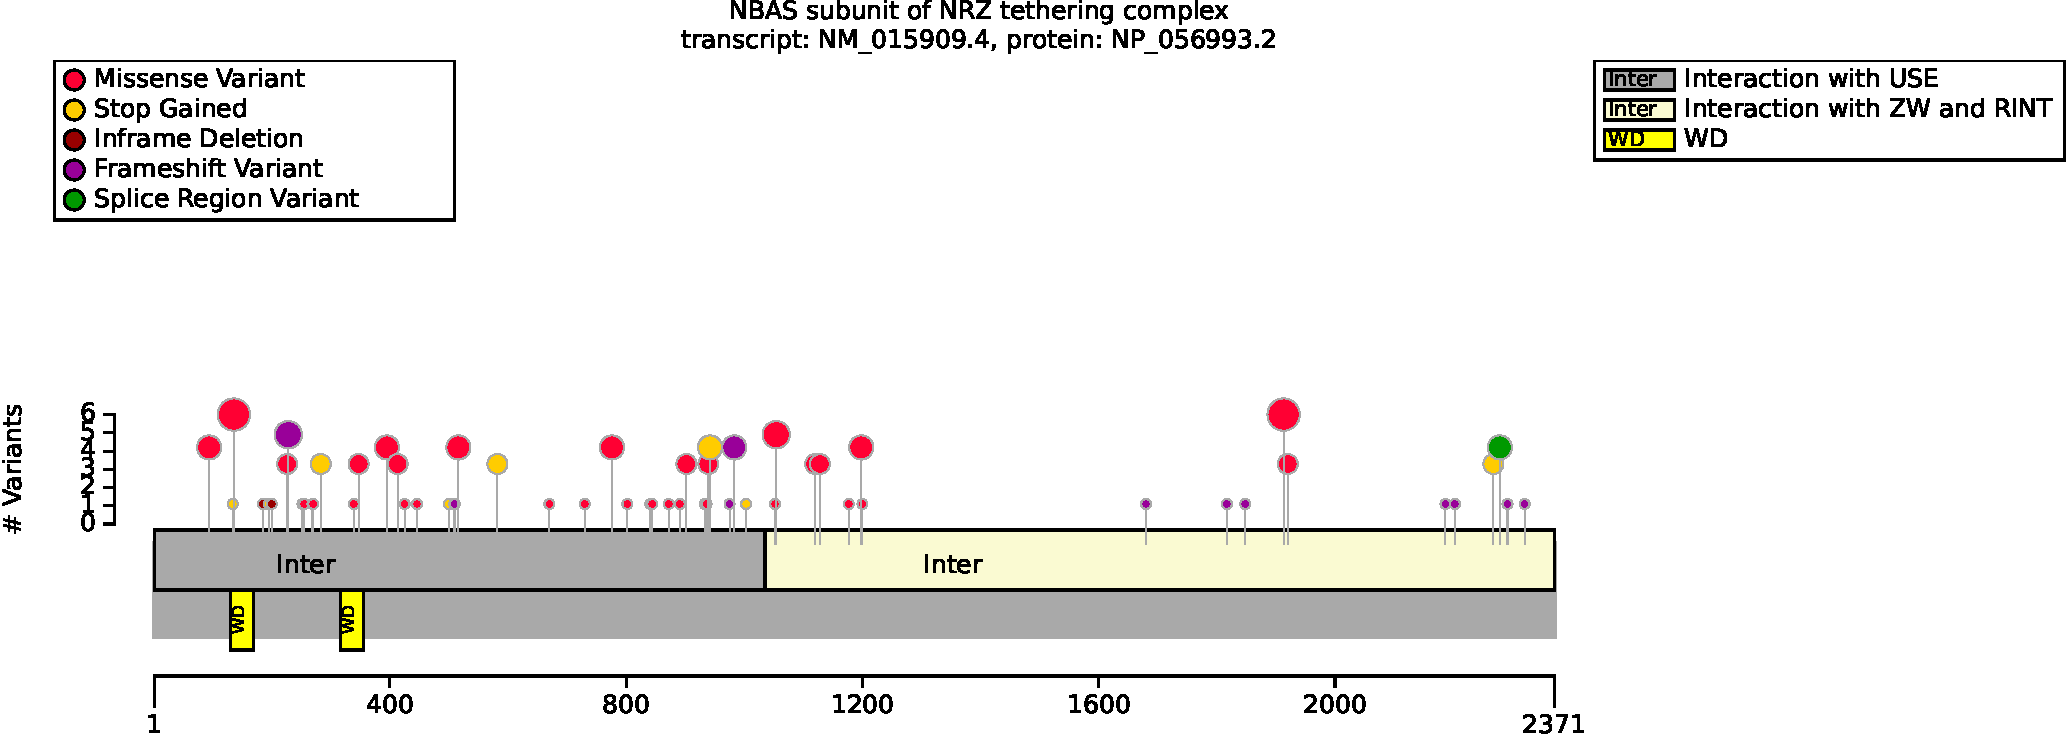
\includegraphics[width=\textwidth]{ img/NBAS_protein_diagram.pdf} 
\captionsetup{justification=raggedright,singlelinecheck=false}
\caption{Distribution of variants in NBAS}
\end{subfigure}
\begin{subfigure}[b]{0.48\textwidth}
\centering
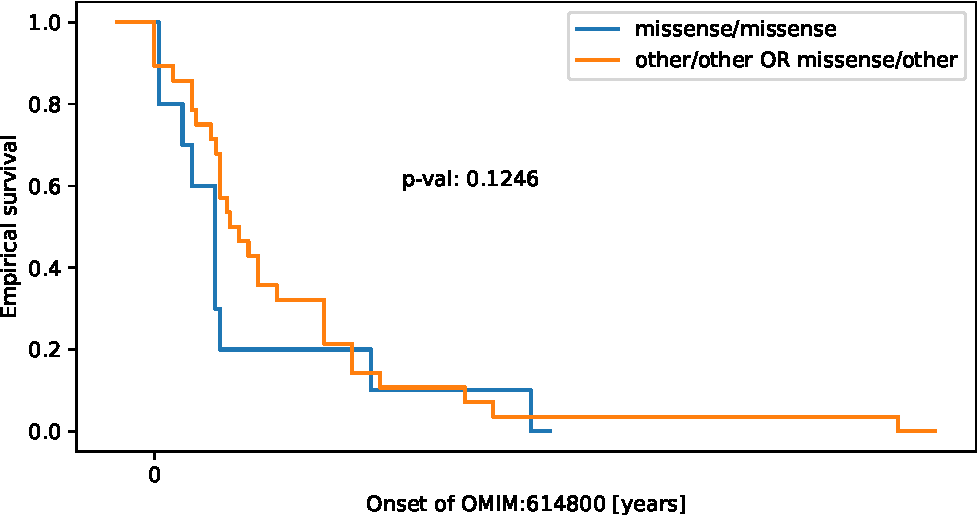
\includegraphics[width=\textwidth]{ img/NBAS_stats.pdf} 
\captionsetup{justification=raggedright,singlelinecheck=false}
\caption{NBAS missense variants vs. age at death.}
\end{subfigure}

\vspace{2em}

\begin{subfigure}[b]{0.95\textwidth}
\centering
\resizebox{\textwidth}{!}{
\begin{tabular}{llllrr}
\toprule
HPO term & missense/missense & other/other OR missense/other & p-value & adj. p-value\\
\midrule
Decreased circulating IgG concentration [HP:0004315] & 1/12 (8\%) & 15/23 (65\%) & 0.002 & 0.019\\
\bottomrule
\end{tabular}
}
\captionsetup{justification=raggedright,singlelinecheck=false}
\caption{Fisher Exact Test performed to compare HPO annotation frequency with respect to missense/missense and other/other OR missense/other. Total of
        12 tests were performed. }
\end{subfigure}
\vspace{2em}
\begin{subfigure}[b]{0.95\textwidth}
\centering
\resizebox{\textwidth}{!}{
\begin{tabular}{llllrr}
\toprule
HPO term & missense/missense & other/other OR missense/other & p-value & adj. p-value\\
\midrule
Decreased circulating IgG concentration [HP:0004315] & 1/12 (8\%) & 15/23 (65\%) & 0.002 & 0.019\\
\bottomrule
\end{tabular}
}
\captionsetup{justification=raggedright,singlelinecheck=false}
\caption{Fisher Exact Test performed to compare HPO annotation frequency with respect to missense/missense and other/other OR missense/other. Total of
        12 tests were performed. }
\end{subfigure}
\vspace{2em}
\begin{subfigure}[b]{0.95\textwidth}
\captionsetup{justification=raggedright,singlelinecheck=false}
\resizebox{\textwidth}{!}{
\begin{tabular}{llllrr}
\toprule
Description & Variable & Genotype (A) & Genotype (B) & p-value & xrefs\\
\midrule
Age of death & Age of death & missense/missense & other/other OR missense/other & 0.125 & -\\
\bottomrule
\end{tabular}
}
\caption{ Age of death to compare missense/missense and other/other OR missense/other with respect to Age of death. }
\end{subfigure}

\vspace{2em}

\caption{ The cohort comprised 67 individuals (19 females, 21 males, 27 with unknown sex). 9 of these individuals were reported to be deceased. A total of 134 HPO terms were used to annotate the cohort. Disease diagnosis: Short stature, optic nerve atrophy, and Pelger-Huet anomaly (OMIM:614800). It was reported that missense or in-frame deletions in the C-terminal region of the NBAS gene are associated with  SOPH syndrome (614800), 
missense or in-frame deletions in the Sec30 domain of NBAS are associated with infantile liver failure syndrome type 2 (616483), 
while missense or in-frame deletions in the beta-propeller domain of NBAS are associated with a combined phenotype of multisystem involvement with acute liver failure \cite{PMID_38244286}.
In our dataset, we found an association with  missense or in-frame deletions in the Sec30 with decreased circulating IgG. A similar finding was obtain for missense variants in general.
Due to the small size of our cohort, this finding should be regarded as preliminary.
 A total of 119 unique variant alleles were found in \textit{NBAS} (transcript: \texttt{NM\_015909.4}, protein id: \texttt{NP\_056993.2}).}
\end{figure}
